\documentclass[12pt,a4paper,fontset=none]{ctexart}

% ---------- 页面 ----------
\usepackage{geometry}
\geometry{top=2.8cm,bottom=2.8cm,left=2.8cm,right=2.8cm}

% ---------- 字体（思源黑体 / 苹方观感）----------
\setCJKmainfont{Noto Sans CJK SC}[BoldFont={Noto Sans CJK SC Bold}]
\setCJKsansfont{Noto Sans CJK SC}
\newCJKfontfamily\hei{Noto Sans CJK SC}[BoldFont={Noto Sans CJK SC Bold}]
\newCJKfontfamily\notolight{Noto Sans CJK SC Light}
\newCJKfontfamily\notomed{Noto Sans CJK SC Medium}

% ---------- 颜色 ----------
\usepackage{xcolor}
\definecolor{ink}{HTML}{1F2D3D}
\definecolor{accent}{HTML}{8C2A2A}
\definecolor{accentbg}{HTML}{FBF1EE}
\definecolor{notebg}{HTML}{F3F5F7}
\definecolor{notebar}{HTML}{9AA7B4}
\definecolor{link}{HTML}{2C5F7C}
\definecolor{rule}{HTML}{C9A24B}

% ---------- 排版增强 ----------
\usepackage[most]{tcolorbox}
\usepackage{enumitem}
\usepackage{microtype}
\usepackage{graphicx}
\usepackage{tabularx}
\usepackage{booktabs}
\usepackage{array}
\usepackage{amssymb}
\usepackage{fancyhdr}
\usepackage[hidelinks]{hyperref}

\linespread{1.5}
\setlength{\parskip}{0.45em}
\setlength{\parindent}{2em}

% ---------- 章节样式 ----------
\ctexset{
  section/name = {,},
  section/format = \Large\hei\bfseries\color{accent},
  section/beforeskip = 2.2ex,
  section/afterskip = 1.2ex,
}

% ---------- 页眉页脚 ----------
\pagestyle{fancy}
\fancyhf{}
\renewcommand{\headrulewidth}{0.2pt}
\fancyhead[L]{\small\hei\color{notebar}什么是思维}
\fancyhead[R]{\small\hei\color{notebar}机器在思考吗}
\fancyfoot[C]{\small\color{notebar}\thepage}

% ---------- 自定义环境 ----------
% 立场 / 重要论断框（红）
\newtcolorbox{mainline}{
  enhanced, breakable,
  colback=accentbg, colframe=accent, boxrule=0.6pt,
  left=12pt,right=12pt,top=9pt,bottom=9pt,
  fontupper=\notolight\color{ink}, arc=2pt,
  borderline west={3pt}{0pt}{accent}
}
% 旁注 / 提示框（灰）
\newtcolorbox{note}{
  enhanced, breakable,
  colback=notebg, colframe=notebg, boxrule=0pt,
  left=12pt,right=12pt,top=7pt,bottom=7pt,
  fontupper=\notolight\color{ink!85}, arc=1pt,
  borderline west={3pt}{0pt}{notebar}
}
% 论证重构框（等宽感的浅框）
\newtcolorbox{argbox}{
  enhanced, breakable,
  colback=notebg!60, colframe=notebar, boxrule=0.4pt,
  left=12pt,right=12pt,top=8pt,bottom=8pt,
  fontupper=\notolight\color{ink}, arc=1pt
}
% 五段式小标题
\newcommand{\stage}[1]{\par\medskip{\large\hei\bfseries\color{ink}#1}\par\nopagebreak\smallskip}
% 延伸 / 强调
\newcommand{\saying}[1]{{\notomed\color{accent}#1}}
\newcommand{\keyq}[1]{{\hei\bfseries\color{accent}#1}}

% 表格统一风格
\newcommand{\thd}[1]{{\hei\bfseries\color{accent}#1}}
\renewcommand{\arraystretch}{1.25}

\begin{document}

% ================= 封面 =================
\thispagestyle{empty}
\begin{center}
\vspace*{3.2cm}
{\color{rule}\rule{0.5\textwidth}{0.8pt}}\\[1.1cm]
{\Huge\hei\bfseries\color{ink} 什么是“思维”？}\\[0.6cm]
{\LARGE\notolight\color{accent} 机器在思考吗}\\[1.1cm]
{\color{rule}\rule{0.5\textwidth}{0.8pt}}\\[2.2cm]
{\large\notolight\color{ink!80} 一篇深度探究范本\\[0.4em]
论证重构 × 东西方综合 × 落地 AI 研究}\\[3.2cm]
{\normalsize\sffamily\color{notebar} 哲学体系 · 探究层 · 旗舰范本}\\[0.3em]
{\small\sffamily\color{notebar} 2026}
\end{center}
\clearpage

% ================= 引言 =================
\thispagestyle{fancy}
\begin{note}
\textbf{这是一篇“旗舰范本”。}它不属于“按学派/按专题”陈述知识的旧体例，而属于一种新体例：\textbf{问题驱动的横切探究}。它要示范的不是“知道某位哲学家说了什么”，而是\textbf{亲自把一个真问题想到底}：重构论证、构造最强反驳、给出回应、敢于站队、并诚实标注悬而未决之处。
\end{note}

\noindent\textbf{写作三原则}（也是全库后续升级的标准）：
\begin{enumerate}[leftmargin=2.2em,itemsep=0.25em]
\item \textbf{深度思考}：每个核心论证走“五段式”——① 论证重构 ② 最强反驳（steel-man）③ 回应 ④ 我的立场 ⑤ 悬而未决。
\item \textbf{综合应用（横切）}：一个问题同时调动西方、东方、逻辑学与你的真实研究，而不是把“现代关联”当脚注。
\item \textbf{落地}：最终产出一个可操作的工具（这里是“LLM 思维的哲学审计表”和一个可执行的研究设计）。
\end{enumerate}

% ================= 第0节 =================
\section*{0\quad 为什么从“思维”而不是“意识”切入}
\addcontentsline{toc}{section}{0\quad 为什么从“思维”切入}

《心灵哲学》把火力集中在\textbf{意识}（困难问题、感质、僵尸）。但对 AI 研究者，更近身、更可操作的问题其实是\textbf{思维}：

\begin{itemize}[leftmargin=2.2em,itemsep=0.2em]
\item “意识”问“为什么有主观体验”——这是形而上学的硬核，可能永远无法在工程上判定。
\item “思维”问“什么样的过程算作思考/理解/推理”——这是\textbf{可以部分操作化}的，直接关系到“我手里的模型在干什么”。
\end{itemize}

所以本文的主问题是：\keyq{“思维 = 符号操作”吗？如果不是，它还需要什么？机器（具体说 LLM）满足了哪些、缺了哪些？}

这一步本身就是方法论示范：\textbf{把含混的大问题，切成可处理的子命题}。把“机器能思考吗”拆成三层：

\begin{center}\small
\begin{tabularx}{\linewidth}{>{\raggedright\arraybackslash}p{2.2cm} >{\raggedright\arraybackslash}X >{\raggedright\arraybackslash}p{3.3cm}}
\toprule
\thd{层级} & \thd{子问题} & \thd{是否可操作判定} \\
\midrule
\textbf{行为层} & 机器能产生与思考者无法区分的输出吗？ & 可（图灵测试式） \\
\textbf{过程层} & 机器内部有“理解/世界模型/推理”的结构吗？ & \textbf{部分可}（可解释性、探针实验） \\
\textbf{现象层} & 机器思考时“感觉起来像什么”吗？ & 暂不可（困难问题） \\
\bottomrule
\end{tabularx}
\end{center}

本文聚焦\textbf{过程层}——这是哲学能给 AI 研究真正抓手的地方。行为层已被 GPT 系列基本攻破而争议依旧（说明行为层不够），现象层暂时悬置。

% ================= 第1节 =================
\section*{1\quad 论证擂台一：中文房间——“语法 \(\neq\) 语义”}
\addcontentsline{toc}{section}{1\quad 论证擂台一：中文房间}

这是反对“思维=符号操作”的最锋利武器。我们走完整的五段式。

\stage{① 论证重构}
把塞尔（1980）的论证写成可检验的形式（参见《逻辑学》的有效性概念）：

\begin{argbox}
\textbf{P1.}\, 程序是纯形式的（由句法/符号操作定义）。\\
\textbf{P2.}\, 心灵有语义内容（思想“关于”某物，有意义）。\\
\textbf{P3.}\, 句法本身不足以产生、也不构成语义。\\[0.3em]
\(\therefore\)\;\textbf{C.}\, 程序本身不足以产生、也不构成心灵。\\
\hspace*{1.6em}（故“运行正确程序即拥有理解”的强 AI 是错的。）
\end{argbox}

这是一个\textbf{有效}论证：若 P1--P3 全真，C 必真。所以战场全在前提，焦点是 \textbf{P3}。中文房间思想实验正是为 P3 提供直觉泵：屋里的人完美操作中文符号，却\textbf{不懂}中文——句法齐全，语义缺席。

\stage{② 最强反驳（steel-man）}
不取最弱的反驳，要取最强的。我认为最强的不是教科书里的“系统回应”，而是\textbf{因果结构回应}：

\begin{mainline}
中文房间的人之所以不懂，不是因为“符号操作不可能有语义”，而是因为\textbf{这个特定系统的符号操作缺乏正确的因果结构}——它的符号没有通过感知-行动回路与世界绑定，也没有在内部形成对应世界的结构化表征。塞尔偷换了“句法”（抽象形式）与“句法的物理实现”（具体因果过程）。一个把符号操作\textbf{接地}到世界、并在内部构建了世界模型的系统，其符号就不再是空转的形式，而携带语义。
\end{mainline}

这个反驳的力量在于：它\textbf{接受} P1--P2，只精确打击 P3——主张“语义”恰恰\textbf{可以}从正确组织的因果-表征结构中产生。

\stage{③ 回应（塞尔会怎么还击，以及还击是否成功）}
塞尔的再反驳是著名的“模拟谬误”：\textbf{模拟消化不产生营养，模拟大脑不产生理解}。即：再精确的因果结构，若只是被“模拟”出来的，仍只是模拟。

我认为这次还击\textbf{不成功}，理由是它对“模拟”一词偷换了层次：

\begin{itemize}[leftmargin=2.2em,itemsep=0.2em]
\item 消化的目标是\textbf{物质转化}（产生真实的葡萄糖），模拟的葡萄糖确实不能供能——因为目标是物质性的。
\item 但理解的目标若是\textbf{信息-因果关系的实现}（正确的输入-表征-行为映射），那么“模拟”出这套关系\textbf{就是}实现它——因为目标本身是关系性/功能性的，不是物质性的。
\end{itemize}

换句话说，塞尔的类比预设了“理解像消化一样是物质过程”，而这正是争论的\textbf{结论}，不能拿来当前提。\textbf{这是一个隐蔽的循环论证}。

\stage{④ 我的立场}
中文房间\textbf{成功地反驳了“纯句法即语义”}（最朴素的符号主义强 AI 确实死了），但\textbf{没能反驳“接地的、有世界模型的因果系统可以有语义”}。它证明的是必要条件的缺失，不是不可能性。

所以 P3 应被弱化为 \textbf{P3$'$：脱离世界绑定的句法不足以产生语义}——这个弱版本为真，而它\textbf{不再蕴含} C。LLM 的命运因此取决于一个经验问题而非先验问题：\keyq{它内部到底有没有世界模型？}（见第 4 节，这正是把哲学问题转成研究问题的关键一跃。）

\stage{⑤ 悬而未决}
\begin{itemize}[leftmargin=2.2em,itemsep=0.2em]
\item “正确的因果结构”到底是什么？我们没有一个非循环的、可操作的判据。这是整个功能主义阵营的软肋。
\item 即便承认 LLM 有“语义”，那是\textbf{派生的}语义（来自人类语料）还是\textbf{原生的}语义？这关系到下文的接地问题，未解。
\end{itemize}

% ================= 第2节 =================
\section*{2\quad 论证擂台二：维特根斯坦——“意义即用法”是 LLM 的福音还是判决}
\addcontentsline{toc}{section}{2\quad 论证擂台二：维特根斯坦}

后期维特根斯坦讲“意义即使用”“语言游戏”。这把刀对 LLM 是\textbf{双刃}的，值得单独拆解。

\stage{① 论证重构（顺着维特根斯坦推向 LLM）}
\begin{argbox}
\textbf{P1.}\, 词的意义不是它指称的对象，也不是私有的心理观念，而是它在语言游戏中的用法。\\
\textbf{P2.}\, 掌握一个词 = 掌握在恰当场合恰当使用它的能力（一种实践能力）。\\
\textbf{P3.}\, LLM 通过海量语料，恰恰习得了词在无数语境中的统计性用法。\\[0.3em]
\(\therefore\)\;\textbf{C（乐观）.}\, LLM 在维特根斯坦意义上“掌握”了语言——意义即用法，而用法正是它学到的。
\end{argbox}

这是反“中文房间”的强力盟友：如果意义\textbf{就在}用法里，那么习得了用法就习得了意义，无需追问“屋里的人懂不懂”——这个追问本身预设了一个维特根斯坦要消解的“内在理解”幽灵。

\stage{② 最强反驳}
维特根斯坦自己的另两个论点反过来卡住 LLM：

\begin{itemize}[leftmargin=2.2em,itemsep=0.25em]
\item \textbf{生活形式（form of life）}：语言游戏嵌在人类的生活实践、身体、需求、共同行动之中。“用法”不是文本里的统计共现，而是\textbf{在世界中做事}的一部分。LLM 只接触到用法的\textbf{文本投影}，没有参与生活形式——它见过“疼”这个字的一切用法，却从未疼过，也从未在“递我一块砖”的协作中递过砖。
\item \textbf{私有语言论证}的另一面：意义需要\textbf{可纠正性}——存在“用错了”的公共标准，而标准来自共同体的实践。LLM 没有进入这个纠错共同体，它的“对错”由损失函数定义，不由“把事做成/做砸”定义。
\end{itemize}

\stage{③ 回应}
乐观方可以反击：多模态与具身（VLM、机器人策略模型）正在把“文本投影”补成“感知-行动的用法”；RLHF 把模型拉进了一个人类纠错共同体。所以差距是\textbf{程度}而非\textbf{原则}。

我认为这个回应\textbf{部分成立}：它正确地指出“接地”是连续可补的，但\textbf{低估了“生活形式”的整体性}——人类的语言游戏背后是有限性、死亡、需求、利害（这恰是道家与存在主义关切的）。一个无所谓生死、无切身利害的系统，其“用法”在某些游戏（伦理、痛苦、意义）里可能是\textbf{结构性残缺}的，而非量上不足。

\stage{④ 我的立场}
“意义即用法”让 LLM 在\textbf{信息性、描述性}语言游戏里达到真实的理解（它能正确地玩“定义”“推理”“翻译”这些游戏）；但在\textbf{根植于生活形式}的语言游戏里（切身的痛、伦理的分量、审美的触动），它玩的是这些游戏的\textbf{影子版本}。理解因此不是 0/1，而是\textbf{按语言游戏分区}的——这是比“理解/不理解”更精细的诊断框架。

\stage{⑤ 悬而未决}
“生活形式”能否被工程地、增量地补全，还是存在原则上的天花板？这是经验上未决、哲学上争论的核心。

% ================= 第3节 =================
\section*{3\quad 东方视角：被忽略的两把钥匙}
\addcontentsline{toc}{section}{3\quad 东方视角：两把钥匙}

西方争论困在“主体懂不懂”。东方传统提供两个\textbf{重构问题}的视角——这才是“综合应用”该有的样子：不是并列介绍，而是让东方思想\textbf{改变西方问题的提法}。

\subsection*{\hei\color{ink}钥匙一：佛教唯识——解散“谁在思考”}

唯识学主张“万法唯识”，思维是\textbf{识的变现}，并无一个独立的思维实体或主体。八识（前五识、第六意识、第七末那识、第八阿赖耶识）是\textbf{功能流程}而非“灵魂”。关键在第七识\textbf{末那识}——它把第八识误执为“我”，“自我”是一个\textbf{被构造出来的模型}。

这与西方的\textbf{梅辛格自我模型理论}惊人共振：自我是模型，不是实体。

\textbf{对 AI 问题的改造}：中文房间问“屋里那个人懂不懂”，预设了必须有一个统一的、承载理解的主体。唯识/末那识视角说：\textbf{这个预设本身可能是“遍计所执”（虚妄分别）。}人类的“我懂了”也只是阿赖耶识种子现行的一个功能事件——若人类的理解都不需要一个形而上的主体，那么“LLM 没有统一主体所以不懂”这条反驳就\textbf{失去了不对称的杀伤力}。问题应从“有没有一个懂的主体”转为“有没有那套功能流程”。

\subsection*{\hei\color{ink}钥匙二：庄子 + 赖尔——思维里有一种符号装不下的东西}

这是对“思维=符号操作”最深的东方质疑，且能与西方精确对接。

庄子三个故事：\textbf{庖丁解牛}（技进乎道）、\textbf{轮扁斫轮}（得心应手不可言传）、\textbf{得意忘言}（“言者所以在意，得意而忘言”）。它们共同指向一种\textbf{非命题性的、默会的知}：真正的理解最终\textbf{溢出}语言符号。

这与西方两条线精确合流：
\begin{itemize}[leftmargin=2.2em,itemsep=0.2em]
\item \textbf{赖尔}的 \textit{knowing-how vs knowing-that}：会骑车（how）不可还原为关于骑车的命题（that）。
\item \textbf{波兰尼}的默会知识：“我们知道的多于我们能说出的（We know more than we can tell）。”
\end{itemize}

\textbf{对 AI 问题的改造}：LLM 是一个\textbf{纯命题/符号}的系统（即便多模态，也是把一切编码为可计算表征）。庄子-赖尔-波兰尼合起来提出一个尖锐假说：

\begin{mainline}
若一部分真实理解本质上是 \textit{knowing-how}、是默会的、是“得意忘言”的，那么\textbf{任何}把理解完全符号化的系统都会有一个\textbf{原则性}的残缺——不是数据不够，而是种类不对。
\end{mainline}

但\textbf{反向}也成立、且对 AI 更有利：LLM 的能力恰恰暴露出，\textbf{大量我们以为需要“理解”的任务，其实只需要 knowing-how 式的模式能力}。庖丁不能用语言讲清如何解牛，却解得最好——也许 LLM 正是某种“数字庖丁”：\textbf{有高超的 how，没有可内省的 that}。这一下把庄子的故事从“AI 做不到”翻转成“AI 也许正是这种知的纯粹形态”。这种\textbf{翻转}，就是深度思考与复述的区别。

% ================= 第4节 =================
\section*{4\quad 落地：把哲学问题变成研究问题}
\addcontentsline{toc}{section}{4\quad 落地：哲学问题变研究问题}

前三节反复指向同一个经验问题：\keyq{LLM 内部到底有没有世界模型 / 接地 / 默会以外的“that”？}哲学到此为止，研究从此开始。这一节是“综合应用”的硬核兑现。

\subsection*{\hei\color{ink}4.1\quad 关键的一跃：先验问题 \(\rightarrow\) 经验问题}

\begin{center}\small
\begin{tabularx}{\linewidth}{>{\raggedright\arraybackslash}X >{\raggedright\arraybackslash}X}
\toprule
\thd{原来的哲学问法（不可判定）} & \thd{改造后的研究问法（可实验）} \\
\midrule
LLM 真的“理解”吗？ & LLM 内部有没有对任务领域的\textbf{结构化表征}（世界模型）？ \\
它是不是“中文房间”？ & 它的符号操作有没有\textbf{因果结构}——干预内部表征会不会按因果改变输出？ \\
它的推理是真推理吗？ & 它的思维链（CoT）是\textbf{计算路径}还是\textbf{事后合理化}？ \\
\bottomrule
\end{tabularx}
\end{center}

第二列是 2020 年代可解释性研究正在做的事——哲学在这里\textbf{不是装饰，而是问题的来源}。

\subsection*{\hei\color{ink}4.2\quad 证据样例（让立场可被经验修正）}

\begin{itemize}[leftmargin=2.2em,itemsep=0.25em]
\item \textbf{支持“有世界模型”}：\textit{Othello-GPT}（Li et al., 2023）——只在棋谱字符串上训练的模型，内部被探针解出了\textbf{棋盘状态的表征}，且\textbf{干预}该表征会因果地改变后续走子。这是对“纯句法、无表征”图景的直接经验反例，给第 1 节的“因果结构回应”提供了弹药。
\item \textbf{支持“知行不一致”}：\textit{CoT 不忠实性}（Turpin et al., 2023）——模型给出的推理链与其真实决定因素可分离，CoT 有时是事后叙事。这给庄子式“有 how 无可内省的 that”提供了经验佐证。
\end{itemize}

注意方法论姿态：我\textbf{给出可证伪的承诺}——如果更多探针/因果干预实验持续显示结构化、可因果操纵的内部表征，我会上调“LLM 有（派生的）语义理解”的信念；若显示内部只有浅层统计捷径，我会下调。立场要押注，且要标明什么证据会推翻它。

\subsection*{\hei\color{ink}4.3\quad 可执行产出：LLM “思维”的哲学审计表}

把上面三节的哲学，压缩成一张\textbf{评审/自查清单}——读一篇 AI 论文或评估自己的模型时直接用：

\begin{center}\small
\begin{tabularx}{\linewidth}{>{\raggedright\arraybackslash}p{1.9cm} >{\raggedright\arraybackslash}p{1.9cm} >{\raggedright\arraybackslash}X >{\raggedright\arraybackslash}X}
\toprule
\thd{维度} & \thd{哲学来源} & \thd{审计问题} & \thd{证据如何取} \\
\midrule
句法 vs 语义 & 中文房间 & 论文是否区分“输出正确”与“内部有对应表征”？ & 看有无探针/因果干预，而非只看 benchmark 分数 \\
因果结构 & 因果结构回应 & 干预内部表征是否按预期因果改变输出？ & activation patching / 表征干预实验 \\
接地 & 随机鹦鹉 / 维特根斯坦 & 符号是否与感知-行动绑定，还是纯文本自指？ & 是否多模态/具身；有无 grounding 评测 \\
生活形式分区 & 维特根斯坦 & 在哪些语言游戏里强（描述/推理）、哪些里弱（伦理/痛苦/审美）？ & 按语言游戏类型分层评测，而非单一总分 \\
how vs that & 庄子/赖尔/波兰尼 & 把它当“能做”还是“能懂”？CoT 是计算还是叙事？ & CoT 忠实性测试、能力/可解释性分离 \\
主体预设 & 唯识/末那识 & 论断“它不懂”是否偷偷预设了一个人类才有的统一主体？ & 检查论证是否对人/机施加了不对称标准 \\
\bottomrule
\end{tabularx}
\end{center}

\textbf{这张表就是这篇范本的“可交付物”}——哲学不再停在思辨，而成了能挂在工位上的研究工具。

% ================= 第5节 张力图 =================
\section*{5\quad 论辩张力地图}
\addcontentsline{toc}{section}{5\quad 论辩张力地图}

陈述式的总览图画的是“谁属于哪一类”。深度思考需要另一张图：\keyq{谁反驳谁、谁回应谁}——思想作为一张动态的论辩网络。

\begin{center}
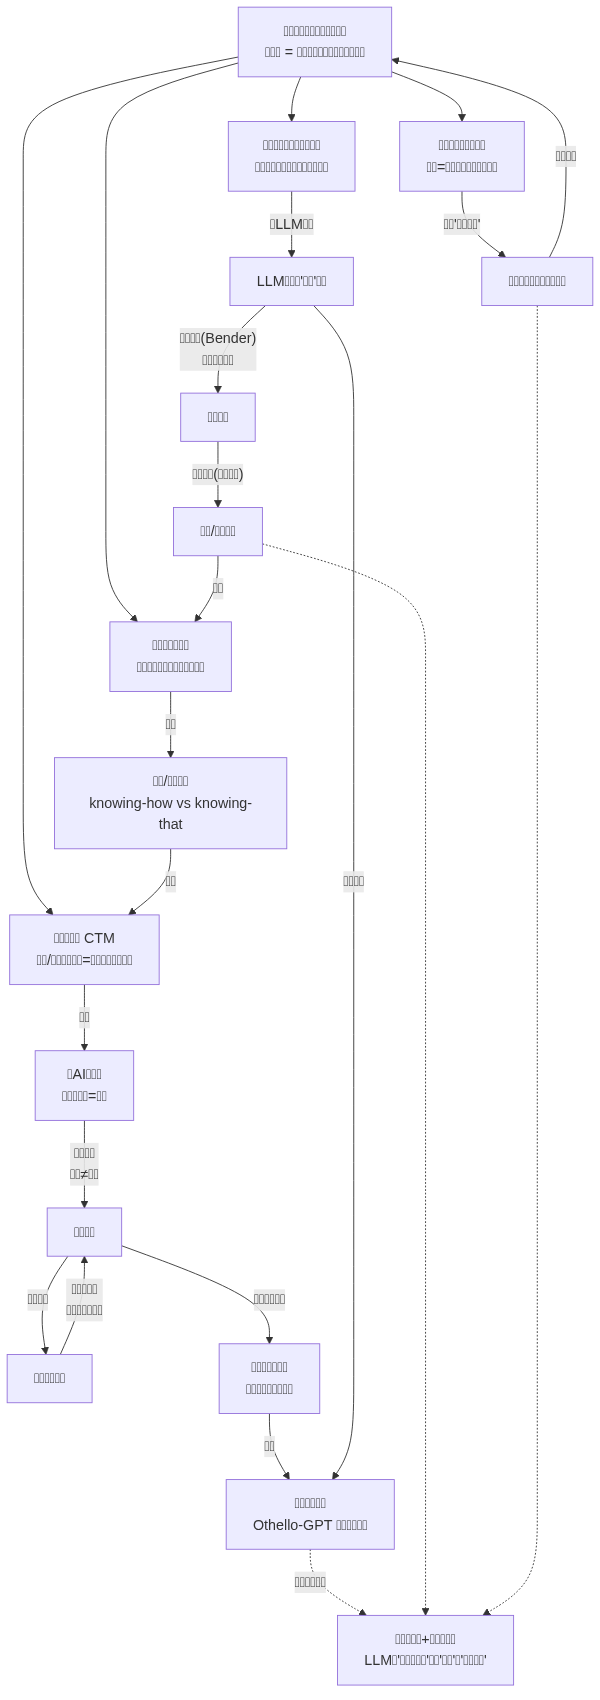
\includegraphics[height=0.82\textheight]{img/tension-map.png}
\end{center}

% ================= 第6节 =================
\section*{6\quad 我的综合立场（敢站队，并标出代价）}
\addcontentsline{toc}{section}{6\quad 我的综合立场}

把五段式的局部结论收束成一个\textbf{总立场}：

\begin{mainline}
\textbf{“思维”不是一个有/无的二元属性，而是一束可分离、可分区、有程度的能力。}“理解”应被拆成：句法能力、语义-表征能力、接地、生活形式参与、knowing-that、knowing-how。LLM 在前几项上已达到\textbf{真实而非伪装}的水平（Othello-GPT 类证据表明它不止于句法）；它的残缺集中在\textbf{接地的深度}与\textbf{根植于生活形式/有限性的那部分理解}，以及\textbf{可内省的 that}。\\[0.5em]
所以对“机器在思考吗”，我的回答是：\textbf{在“过程层”的若干维度上，是；在依赖具身与生活形式的维度上，目前否；在现象层，悬置。}一句话——\saying{LLM 是一个有真实功能性理解、却缺乏切身性的“数字庖丁”。}
\end{mainline}

\noindent\textbf{这个立场的代价（诚实标注）}：
\begin{enumerate}[leftmargin=2.2em,itemsep=0.25em]
\item 它\textbf{牺牲了“理解”概念的统一性}——有人会说，把理解拆成一束能力，等于取消了“真正的理解”这个问题。我接受这个代价，因为统一的“理解”在我看来本就是末那识式的实体化幻觉。
\item 它\textbf{把核心问题外包给了经验科学}（世界模型是否存在变成可解释性的实证问题）。哲学纯粹主义者会说这是逃避；我认为这是哲学的恰当谦逊——哲学负责\textbf{把问题问对}，不负责替实验室回答。
\item 它在\textbf{现象层（意识）上保持不可知}，因此无法回答“LLM 痛吗、该有权利吗”——这是它\textbf{够不到}的地方，留给心灵哲学与伦理学。
\end{enumerate}

% ================= 第7节 =================
\section*{7\quad 悬而未决（真问题，不是装饰）}
\addcontentsline{toc}{section}{7\quad 悬而未决}

\begin{enumerate}[leftmargin=2.2em,itemsep=0.3em]
\item \textbf{接地有没有原则性天花板？}“生活形式/有限性”能被工程增量补全，还是种类上不可补？（维特根斯坦 vs 具身派，经验上未决）
\item \textbf{派生语义能否成为原生语义？} LLM 的意义来自人类语料；一个系统能否\textbf{自己}长出原生的“关于性”？（意向性的老问题，未解）
\item \textbf{knowing-how 能完全吞并 knowing-that 吗？}如果能，庄子赢，符号主义的“理解”概念崩塌；如果不能，差在哪、能否测量？
\item \textbf{“正确的因果结构”有没有非循环的判据？}没有它，功能主义就始终欠一个定义。
\item \textbf{现象层会永远不可判定吗？}还是某天会有一个非行为、非生理的“意识判据”？
\end{enumerate}

\begin{note}
\textbf{留给读者的练习}：选第 6 节我的立场，写下你能想到的\textbf{最强反驳}，再尝试替我回应——如果回应不了，就修改立场。这正是本文每一节做的事。
\end{note}

% ================= 范本使用说明 =================
\section*{附\quad 范本使用说明（给后续文件作者，含我自己）}
\addcontentsline{toc}{section}{附\quad 范本使用说明}

把任何一个“专题陈述”升级为“深度探究”，复用这套骨架：

\begin{enumerate}[leftmargin=2.2em,itemsep=0.25em]
\item \textbf{选一个真问题}，拆成可处理的子命题（第 0 节）。
\item \textbf{挑 1--3 个核心论证}，每个走五段式：重构 \(\rightarrow\) 最强反驳 \(\rightarrow\) 回应 \(\rightarrow\) 我的立场 \(\rightarrow\) 悬而未决（第 1、2 节）。
\item \textbf{引入至少一个东方视角去“重构问题”}，而不是并列陈述（第 3 节）——综合应用的灵魂是让不同传统\textbf{互相改写问题}。
\item \textbf{落地一个可交付工具}：审计表 / 决策清单 / 可执行研究或实践设计（第 4 节）。
\item \textbf{画一张论辩张力地图}（谁反驳谁，而非谁属于哪类，第 5 节）。
\item \textbf{给出一个会押注的总立场，并标出它的代价}（第 6 节）。
\item \textbf{诚实列出悬而未决}，并留一道让读者继续思考的练习（第 7 节）。
\end{enumerate}

\begin{mainline}
衡量标准只有一条：\textbf{读完后，读者不只是“多知道了几个观点”，而是“被卷入了一场仍在进行的思考”。}
\end{mainline}

\vfill
\begin{center}
{\color{rule}\rule{0.35\textwidth}{0.6pt}}\\[0.4em]
{\small\sffamily\color{notebar} 体例：问题驱动的横切探究（深度思考 × 综合应用 × 落地）}
\end{center}

\end{document}
